\chapter{Aplicando Análise Temporal}
\label{chap:aplicando}

Neste capítulo, vemos entender como a análise temporal pode ser aplicado em cima dos dados coletados durante a análise exploratória tanto no contexto espacial, quanto no contexto de domínio.

\section{Contexto Espacial}

O contexto espacial se refere aos aspectos geográficos como, por exemplo, em que parte da cidade o analista se interessa.

\begin{figure}[t]
	\centering
	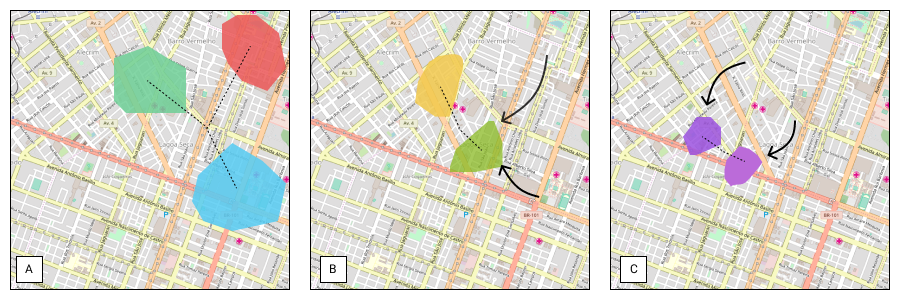
\includegraphics[width=\textwidth]{imagens/analise-contexto-espacial}
	\caption{Evolução no contexto espacial.}
	\label{fig:analise-contexto-espacial}
\end{figure}

\section{Contexto de Domínio}

O contexto de domínio se refere aos aspectos de domínio como, por exemplo, se o analista tem mais interesse em casas com varanda ou apartamentos.